\subsection{Anzeigen aller Stationen}
\label{sub:anzeigen_aller_stationen}

  Nachdem zuvor alle Trips mit ihren Polylines in der Karte angezeigt wurden, folgt nun das Anzeigen aller Stationen, die zu einem Trip gehören. Änlich wie beim Abfragen und Anzeigen aller Polylines, sollte dieser Schritt mögliche Engpässe oder unvorhergesehene Probleme aufdecken (Abbildung \ref{fig:prozess/draw_all_stations}).

  \begin{figure}[htbp]
     \begin{center}
       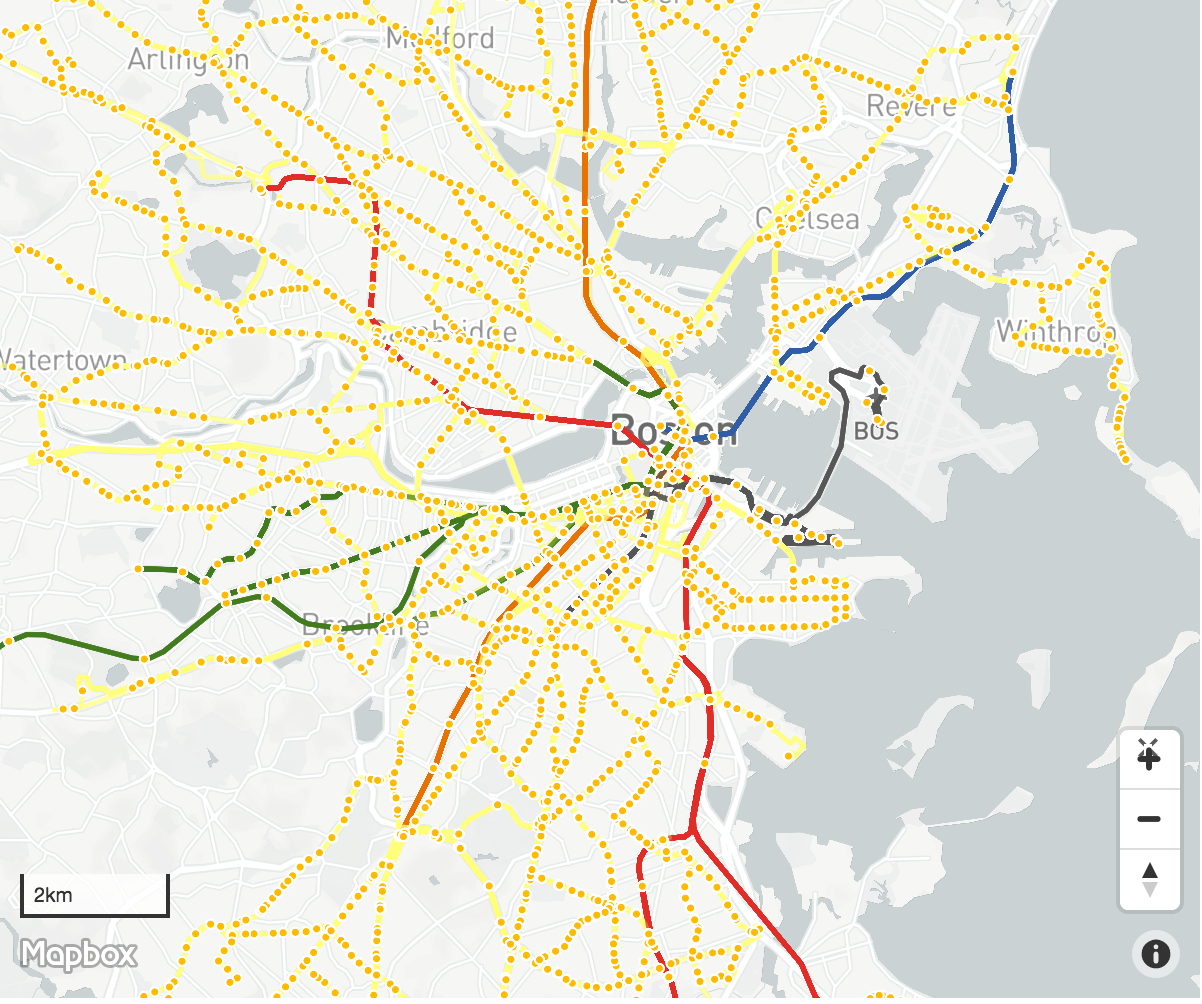
\includegraphics[width=0.6\textwidth]{prozess/draw_all_stations}
       \caption{Aktive Trips mit ihren dazugehörenden Stationen}
       \label{fig:prozess/draw_all_stations}
     \end{center}
   \end{figure}
   
  Vor allem die Abfrage von aktiven Trips aus der Datenbank, stellte ein großes Problem dar. Die Datenbank konnte die Anfragen des Clients nicht effizient genug verarbeiten. An dieser Stelle stand fest, dass für die weitere Arbeit umfassende Optimierungen der Datenbank erfolgen müssen, um eine responsive Webanwendung zu ermöglichen. 

  \subsubsection{GTFS Optimierungen}
  \label{ssub:gtfs_optimierungen}
    Der erste Schritt um die Performance zu verbessern, ist die Optimierung von GTFS Feeds. Damit lässt sich die Datenmenge bereits vor dem Importieren in die Datenbank, erheblich verringern. Ein Tool um ein GTFS Feed umfassend zu optimieren ist \texttt{gtfstidy} \url{https://github.com/patrickbr/gtfstidy}. Es bietet dabei allerdings nicht nur die Möglichkeit für die Vereinfachung von Polylines sondern kommt mit einer ganzen Reihe an Optimierungsmöglichkeiten. 

    Der Kommandozeilenbefehl \colorbox{materialGrey}{\texttt{\color{white}{\$ gtfstidy -sSiRDeO input.zip output}}} optimiert das Stuttgart-VVS Feed wie folgt:
    
    \begin{itemize}[label={}]
      \item \textbf{-s} Reduziert die Punktanzahl einer Polyline
        
      \item \textbf{-S} Entfernt redundante Polylines.

      \item \textbf{-i} Umwandlung von Zeichen ID's (String) in Zahlen ID's (Integer).\footnote{Aus der String ID \texttt{'1.T0.10-1-j17-1.16.H'} wird \texttt{78}}

      \item \textbf{-O} Entfernt Feed Einträge die nicht referenziert werden.

      \item \textbf{-R} Entfernt doppelt vorhandene Routen.

      \item \textbf{-e} Setzt fehlerhafte oder optionale Felder auf einen Standard Wert.

      \item \textbf{-D} Entfernt fehlerhafte Einträge aus dem Feed.
    \end{itemize}

    Durch Verwendung von gtfstidy konnte das Feed optimiert werden und die Datengröße der einzelnen Dateien um folgendes Maß verringert werden.

    \begin{longtable}{|>{\raggedright \arraybackslash}p{5.0cm}|>{\raggedright \arraybackslash}p{5.0cm}|>{\raggedright \arraybackslash}p{5.0cm}|}
      \hline
      Dateiname & Größe davor& Größe danach\\
      \hline
      trips.txt & 6 MB & 2.8 MB\\
      stop\_times.txt & 103 MB & 53 MB\\
      stops.txt & 651 KB & 355 KB\\
      shapes.txt & 77.3 MB & 22.4 MB\\
      routes.txt & 54 KB & 38 KB\\
      calendar\_dates.txt & 557 KB & 463 KB\\
      \hline
      \caption{Tabellengröße bevor und nach anwenden von gtfstidy}
      \label{tbl:gtfs_tidy_results}
    \end{longtable}

    Insgesamt konnte so die Größe des Feeds von 79 MB auf 118 MB um knapp 50\% verringert werden. Vor allem die Umwandlung von langen String ID's in kürzere Integer ID's trägt maßgeblich zur Verringerung der Dateigröße bei.

  % subsubsection gtfs_optimierungen (end)

  \subsubsection{Denormalisierung der Datenbank}
  \label{ssub:denormalisierung_der_datenbank}
    Die Denormalisierung ist eine Strategie, die auf eine zuvor normalisierte Datenbank angewendet wird, um die Leistung zu erhöhen. Die Denormalisierung ist der Prozess, bei dem versucht wird, die Leseperformance einer Datenbank zu verbessern, auf Kosten der Schreibleistung, durch Hinzufügen redundanter Kopien von Daten oder durch deren Gruppierung.\parencite{sanders}
    Der große Nachteil von Denormalisierung, nämlich die Redundanz von Daten, spielt für dieses Projekt keine Rolle, da die Daten ausschließlich ausgelesen und nicht geschrieben werden. Was bleibt sind die Vorteile.\\

    Für dieses Projekt bedeutet diese Methode, eine neue Tabelle zu generieren, die den Zugriff auf die benötigten Daten einfach macht. Im Grunde handelt es sich um eine Vorberechnung. Anstatt die Tabellen bei jeder Anfrage an den Server aufwendig über viele \texttt{SQL-JOINS} zu verknüpfen, wird diese Verknüpfungen einmalig vorberechnet und in eine Tabelle gespeichert. Eine Denormalisierung  einer Tabelle ist bereits im vorherigen Abschnitt "`\nameref{ssub:aggregieren_der_shape_tabelle}"' gezeigt und führte dazu, dass die Polyline über die Abfrage einer einzigen Tabellenreihe erhalten werden kann was die Performance signifikant erhöhte. Zur besseren Verständnis soll folgende Grafik helfen:

    \begin{figure}[htbp]
      \begin{center}
        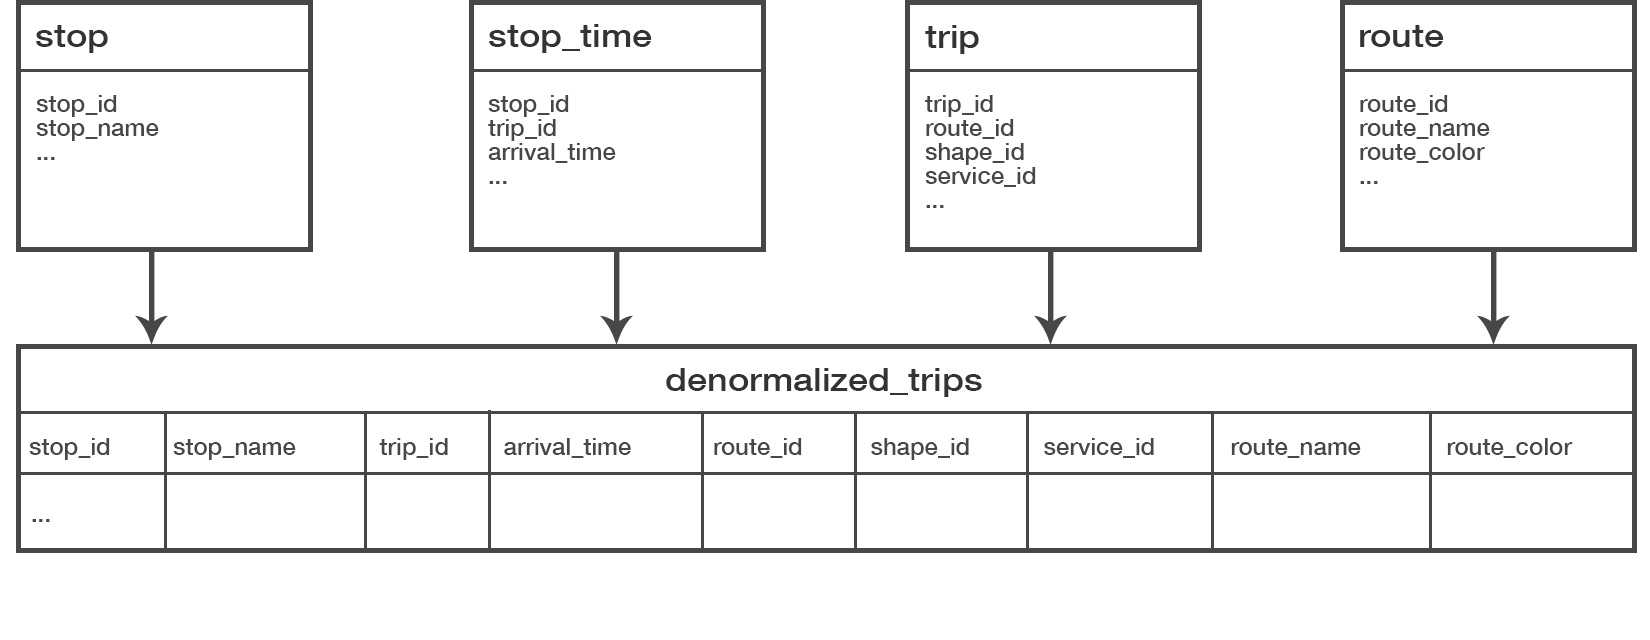
\includegraphics[width=\textwidth]{denormalizing.jpg}
        \caption{Beispiel einer Denormalisierung von Tabellen}
        \label{fig:denormalizing}
      \end{center}
    \end{figure}

    Wie in Abbildung \ref{fig:denormalizing} zu sehen ist, wird aus einer vertikalen Anordnung der einzelnen Datenfelder, eine horizontale Anordnung in einer einzigen \texttt{denormalized\_trips} Tabelle. Eine Reihe in dieser neuen Tabelle steht für genau einen Eintrag eines Trips. Anstatt also bei jeder Anfrage an den Server die verschiedenen Daten mittels \texttt{JOIN} verknüpfen zu müssen, können diese jetzt per Zugriff auf eine einzige Reihe in nur einer Tabelle erfragt werden.

    Dieses Prinzip, der Gruppierung von Daten in einer neuen Tabelle soll nun auch auf die anderen benötigten Tabellen angewendet werden. Die Denormalisierung erfolgt in 3 Schritten:

    \begin{enumerate}
      \item Erstellen der neuen Tabelle \texttt{denormalized\_trips}
      \item Importieren der verschiedenen Daten in diese neue Tabelle
      \item Mögliche Abfragen sind nun über diese neue Tabelle möglich.
    \end{enumerate}

    Das SQL-Statement ist abermals aufgrund seiner Länge Anhang \ref{lst:denormalized_shapes} zu entnehmen. Dies resultiert in einer Tabelle die wie folgt aussieht:

    \begin{figure}[htbp]
      \begin{center}
        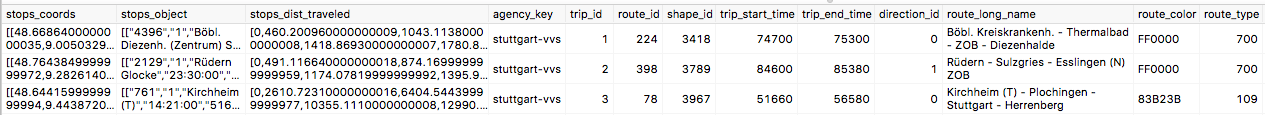
\includegraphics[width=\textwidth]{denormalized_tables.png}
        \caption{Auszug aus der \texttt{denormalized\_trips} Tabelle}
        \label{fig:denormalized_table}
      \end{center}
    \end{figure}  

    \subsubsection*{Ergebnisse der Denormalisierung}
    \label{ssub:ergebnisse_der_denormalisierung}
      Für die Visualisierung ist eine Abfrage der aktiven Trips am wichtigsten.
      Folgende Tabellen werden für die Abfrage benötigt.

      \begin{figure}[htbp]
        \begin{center}
          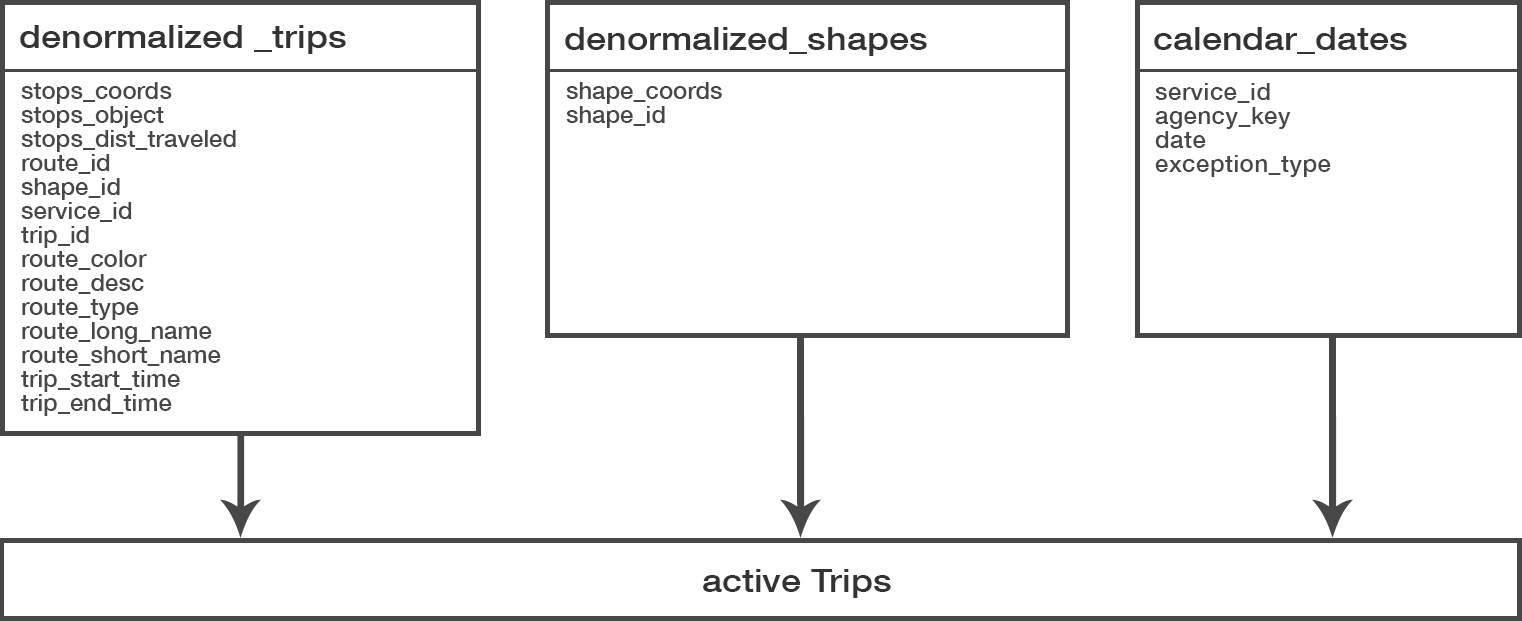
\includegraphics[width=\textwidth]{denormalizing_results.jpg}
          \caption{Benötigte Tabellen zur Abfrage von Trips}
          \label{fig:denormalizing_results}
        \end{center}
      \end{figure}

      Wie zu sehen ist, wird auf die Denormalisierte \texttt{Shape} und \texttt{Trips} Tabelle zugegriffen.

      Nachfolgend die Ergebnisse für die Abfrage von Trips in einem wachsenden Zeitrahmen. Die verwendete SQL-Abfrage befindet sich im \nameref{sec:anhang} unter Listing \ref{lst:query_trips}.

      \begin{longtable}{|>{\raggedright \arraybackslash}p{5.0cm}|>{\raggedright \arraybackslash}p{5.0cm}|>{\raggedright \arraybackslash}p{4.0cm}|}
      \caption{Evaluierung der Denormalisierung}\label{tbl:evaluierung_der_denormalisierung}\\
        \hline
          Zeitraum & Trip Anzahl & Query Zeit\\
        \hline
          9:00 bis 9:15 & 88 & 98 ms\\
          9:00 bis 10:00 & 1125 & 154 ms\\
          9:00 bis 12:00 & 3360 & 285 ms\\
          9:00 bis 15:00 & 7070 & 497 ms\\
          9:00 bis 21:00 & 14718 & 900 ms\\
        \hline
      \end{longtable}

      Die Ergebnisse Zeigen, dass die Abfragezeit der Datenbank für die aktiven Trips erheblich gesunken ist. Anfangs ist solch eine Anfrage aufgrund der endlosen Laufzeit erst gar nicht möglich gewesen.

      \begin{figure}[htbp]
        \begin{center}
          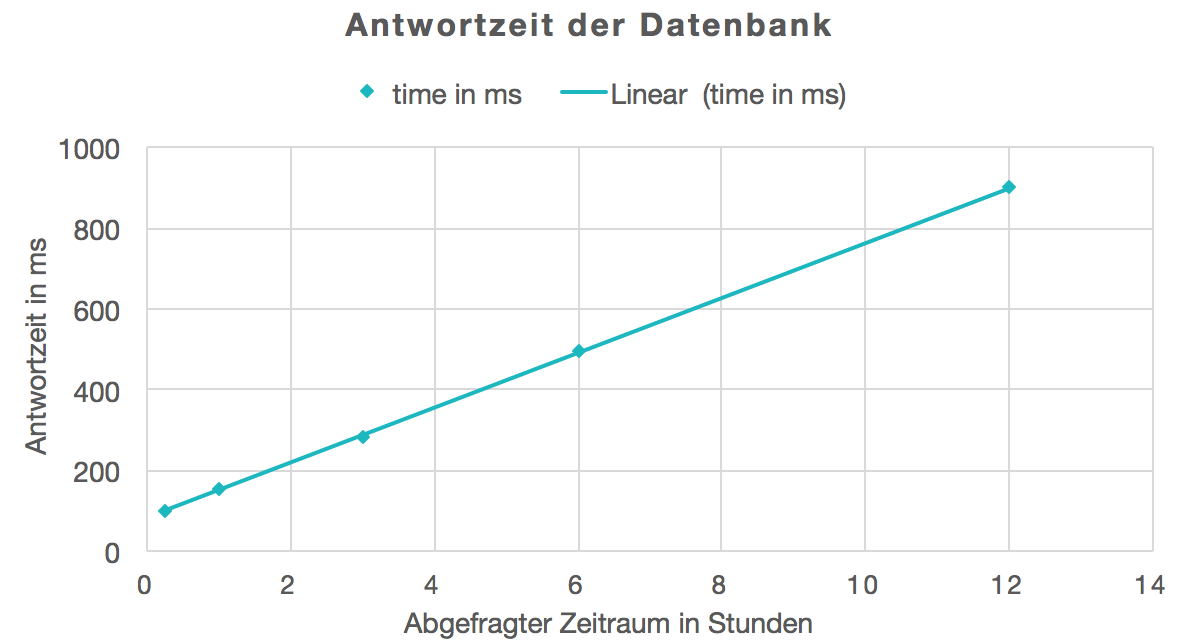
\includegraphics[width=0.7\textwidth]{query_time_chart}
          \caption{Plot der Abfragezeiten}
          \label{fig:query_time_chart}
        \end{center}
      \end{figure}
      
      Abbildung \ref{fig:query_time_chart} zeigt einen Plot der Query Zeit aus Tabelle \ref{tbl:evaluierung_der_denormalisierung} als linearen Graphen. Daraus folgt, dass die Antwortzeit der Datenbank linear mit dem abgefragten Zeitraum wächst. Für die Visualisierung sind vor allem zwei Abfragen wichtig: Erstens das Abfragen eines größeren Zeitraums von 1-2 Stunden. Dies geschieht beim ersten Aufrufen der Webanwendung wenn die Karte noch keine Trips besitzt und damit leer ist. Zweitens die Abfrage von nur kleinen Zeiträumen von nur einer Minute, um neue Trips abzufragen. Für diese zwei Abfragen bewegt sich die Antwortzeit des Servers zwischen $\approx 80 -  160\; ms$. Damit wurde das in Kapitel \ref{sub:zielsetzung} gesetzte ziel von 0 bis $200ms$ bereits erreicht.
      
    % subsubsection ssub:ergebnisse_der_denormalisierung (end)
  % subsubsection denormalisierung_der_datenbank (end)
% subsection anzeigen_aller_stationen (end)